\documentclass{article}

% packages
\usepackage{amsmath, amsthm, thmtools, amsfonts, amssymb, luacode, catchfile, tikzducks, hyperref, ifthen}
\ifcsname c@kobocompile\endcsname
	\usepackage[a5paper, total={1072pt, 1448pt}, margin=10pt, includeheadfoot]{geometry} % set page margins
\else
	\usepackage[a4paper, margin=50pt, includeheadfoot]{geometry}
\fi
\usepackage[shortlabels]{enumitem}
\usepackage[skip=3pt, indent=0pt]{parskip}

% language
\usepackage[bidi=basic, layout=tabular, provide=*]{babel}
\ifcsname c@english\endcsname
	\babelprovide[main, import]{english}
\else
	\babelprovide[main, import]{hebrew}
	\babelprovide{rl}
\fi
%\babelfont{rm}{Libertinus Serif}
\babelfont{rm}[Renderer=Harfbuzz]{Libertinus Serif}
\babelfont{sf}{Libertinus Sans}
\babelfont{tt}{Libertinus Mono}

% style
\AddToHook{cmd/section/before}{\clearpage}	% Add line break before section
\linespread{1.3}
\setcounter{secnumdepth}{0}		% Remove default number tags from sections, this won't do well with theorems
\AtBeginDocument{\setlength{\belowdisplayskip}{3pt}}
\AtBeginDocument{\setlength{\abovedisplayskip}{3pt}}
\graphicspath{ {../images/} }

% operators
\DeclareMathOperator\cis{cis}
\DeclareMathOperator\Sp{Sp}
\DeclareMathOperator\tr{tr}
\DeclareMathOperator\im{Im}
\DeclareMathOperator\re{Re}
\DeclareMathOperator\diag{diag}
\DeclareMathOperator*\lowlim{\underline{lim}}
\DeclareMathOperator*\uplim{\overline{lim}}
\DeclareMathOperator\rng{rng}
\DeclareMathOperator\Sym{Sym}
\DeclareMathOperator\Arg{Arg}
\DeclareMathOperator\Log{Log}
\DeclareMathOperator\dom{dom}
\DeclareMathOperator\supp{Supp}
\DeclareMathOperator\var{Var}
\DeclareMathOperator\cov{Cov}

% commands
%\renewcommand\qedsymbol{\textbf{מש''ל}}
%\renewcommand\qedsymbol{\fbox{\emoji{lizard}}}
\newcommand{\Aa}[0]{\mathcal{A}}
\newcommand{\Bb}[0]{\mathcal{B}}
\newcommand{\CC}[0]{\mathbb{C}}
\newcommand{\Cc}[0]{\mathcal{C}}
\newcommand{\EE}[0]{\mathbb{E}}
\newcommand{\FF}[0]{\mathbb{F}}
\newcommand{\Ff}[0]{\mathcal{F}}
\newcommand{\Ii}[0]{\mathcal{I}}
\newcommand{\Gg}[0]{\mathcal{G}}
\newcommand{\Ll}[0]{\mathcal{L}}
\newcommand{\Mm}[0]{\mathcal{M}}
\newcommand{\NN}[0]{\mathbb{N}}
\newcommand{\Nn}[0]{\mathcal{N}}
\newcommand{\PP}[0]{\mathbb{P}}
\newcommand{\Pp}[0]{\mathcal{P}}
\newcommand{\QQ}[0]{\mathbb{Q}}
\newcommand{\RR}[0]{\mathbb{R}}
\newcommand{\Rr}[0]{\mathcal{R}}
\newcommand{\Ss}[0]{\mathcal{S}}
\newcommand{\TT}[0]{\mathbb{T}}
\newcommand{\Uu}[0]{\mathcal{U}}
\newcommand{\Vv}[0]{\mathcal{V}}
\newcommand{\Ww}[0]{\mathcal{W}}
\newcommand{\ZZ}[0]{\mathbb{Z}}
\newcommand{\acts}[0]{\circlearrowright}
\newcommand{\explain}[2] {
	\begin{flalign*}
		 && \text{#2} && \text{#1}
	\end{flalign*}
}
\newcommand{\maketitleprint}[0]{ \begin{center}
	%\begin{tikzpicture}[scale=3]
	%	\duck[graduate=gray!20!black, tassel=red!70!black]
	%\end{tikzpicture}	
	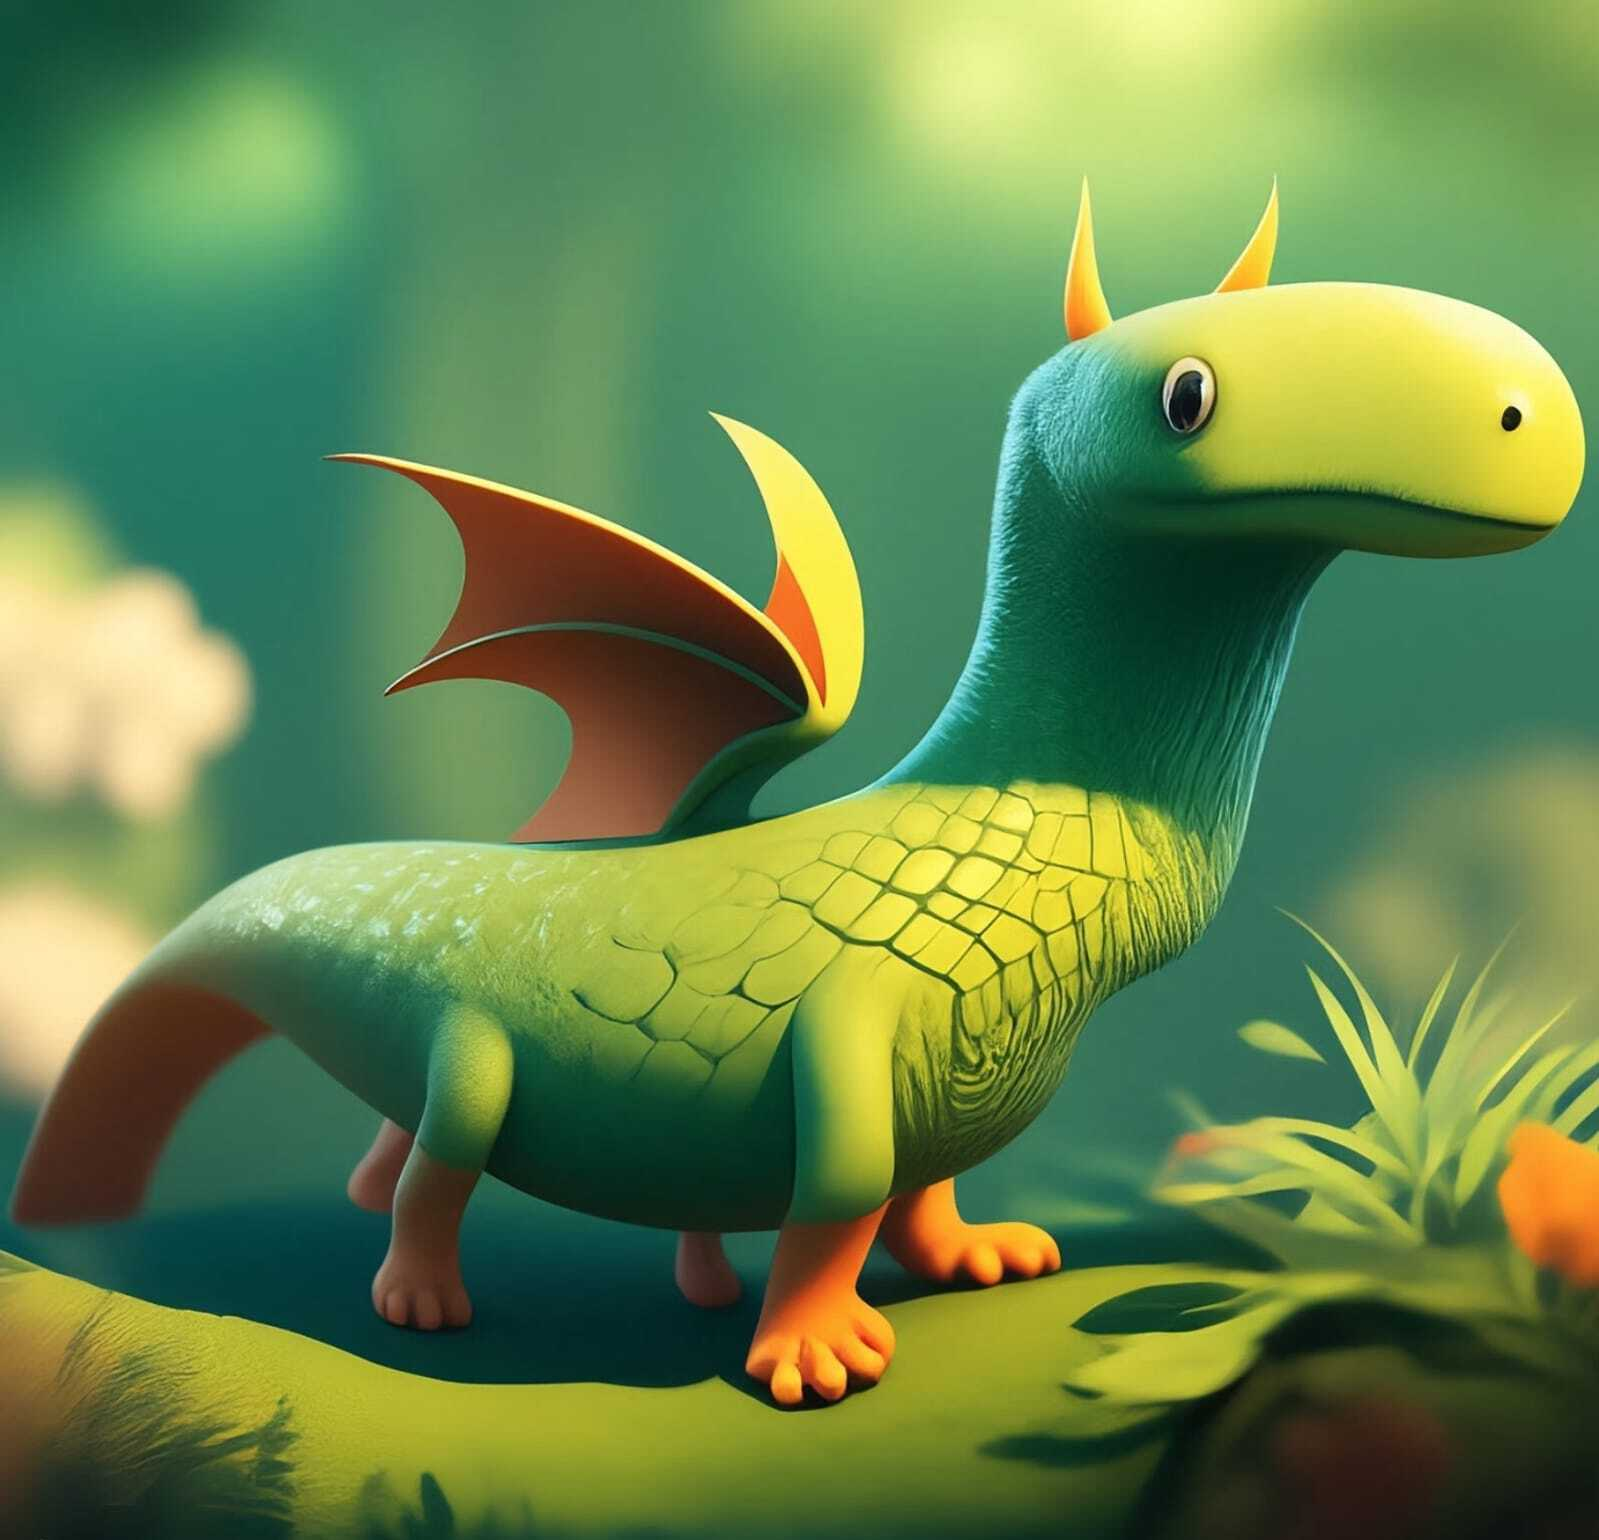
\includegraphics[width=6cm]{cover}
\end{center}
}

% theorem commands
\newtheoremstyle{c_remark}
	{}	% Space above
	{}	% Space below
	{}% Body font
	{}	% Indent amount
	{\bfseries}	% Theorem head font
	{}	% Punctuation after theorem head
	{.5em}	% Space after theorem head
	{\thmname{#1}\thmnumber{ #2}\thmnote{ \normalfont{\text{(#3)}}}}	% head content
\newtheoremstyle{c_definition}
	{3pt}	% Space above
	{3pt}	% Space below
	{}% Body font
	{}	% Indent amount
	{\bfseries}	% Theorem head font
	{}	% Punctuation after theorem head
	{.5em}	% Space after theorem head
	{\thmname{#1}\thmnumber{ #2}\thmnote{ \normalfont{\text{(#3)}}}}	% head content
\newtheoremstyle{c_plain}
	{3pt}	% Space above
	{3pt}	% Space below
	{\itshape}% Body font
	{}	% Indent amount
	{\bfseries}	% Theorem head font
	{}	% Punctuation after theorem head
	{.5em}	% Space after theorem head
	{\thmname{#1}\thmnumber{ #2}\thmnote{ \text{(#3)}}}	% head content

\ifcsname c@english\endcsname
	\theoremstyle{plain}
	\newtheorem{theorem}{Theorem}[section]
	\newtheorem{lemma}[theorem]{Lemma}
	\newtheorem{proposition}[theorem]{Proposition}
	\newtheorem*{proposition*}{Proposition}
	%\newtheorem{corollary}[theorem]{אין חלופה עברית}

	\theoremstyle{definition}
	\newtheorem{definition}[theorem]{Definition}
	\newtheorem*{definition*}{Definition}
	\newtheorem{example}{Example}[section]
	\newtheorem{exercise}{Exercise}[section]

	\theoremstyle{remark}
	\newtheorem*{remark}{Remark}
	\newtheorem*{solution}{Solution}
	\newtheorem{conclusion}[theorem]{Conclusion}
	\newtheorem{notation}[theorem]{Notation}
\else
	\theoremstyle{c_plain}
	\newtheorem{theorem}{משפט}[section]
	\newtheorem{lemma}[theorem]{למה}
	\newtheorem{proposition}[theorem]{טענה}
	\newtheorem*{proposition*}{טענה}
	%\newtheorem{corollary}[theorem]{אין חלופה עברית}

	\theoremstyle{c_definition}
	\newtheorem{definition}[theorem]{הגדרה}
	\newtheorem*{definition*}{הגדרה}
	\newtheorem{example}{דוגמה}[section]
	\newtheorem{exercise}{תרגיל}[section]

	\theoremstyle{c_remark}
	\newtheorem*{remark}{הערה}
	\newtheorem*{solution}{פתרון}
	\newtheorem{conclusion}[theorem]{מסקנה}
	\newtheorem{notation}[theorem]{סימון}
\fi

% Questions related commands
\newcounter{question}
\setcounter{question}{1}
\newcounter{sub_question}
\setcounter{sub_question}{1}

\ifcsname c@english\endcsname
	\newcommand{\question}[1][0]{
		\ifthenelse{#1 = 0}{}{\setcounter{question}{#1}}
		\section{Question \arabic{question}}
		\addtocounter{question}{1}
		\setcounter{sub_question}{1}
	}

	\newcommand{\subquestion}[1][0]{
		\ifthenelse{#1 = 0}{}{\setcounter{sub_question}{#1}}
		\subsection{Part \alph{sub_question}}
		\addtocounter{sub_question}{1}
	}
\else
	\newcommand{\question}[1][0]{
		\ifthenelse{#1 = 0}{}{\setcounter{question}{#1}}
		\section{שאלה \arabic{question}}
		\addtocounter{question}{1}
		\setcounter{sub_question}{1}
	}

	\newcommand{\subquestion}[1][0]{
		\ifthenelse{#1 = 0}{}{\setcounter{sub_question}{#1}}
		\subsection{סעיף \localecounter{letters.gershayim}{sub_question}}
		\addtocounter{sub_question}{1}
	}
\fi

% import lua and start of document
\directlua{common = require ('../common')}

\GetEnv{AUTHOR}

% headers
\author{\AUTHOR}
\date\today

\title{פתרון מטלה 08 --- מבוא לטופולוגיה, 80516}
% chktex-file 9
% chktex-file 17

\begin{document}
\maketitle
\maketitleprint[purple]

\question{}
יהי מרחב טופולוגי $X$ ו־$\beta X$ קומפקיפיקציית סטון־צ'ך.

\subquestion[2]
נניח ש־$X$ דיסקרטי ונראה שאם $U \subseteq \beta X$ פתוחה אז $\cl_{\beta X}(U)$ פתוחה אף היא.
\begin{proof}
	תהי $U$ פתוחה ב־$\beta X$, ויהי $\iota : X \to \beta X$ שיכון כך ש־$\iota(X)$ צפופה ב־$\beta X$. \\
	אם קיימת קבוצה $V \subseteq X$ כך ש־$\iota(V) = U$ אז מהומיאומורפיות לתמונה של $\iota$ נובע ש־$V$ פתוחה.
	הומיאומורפיזם משמר סגור ולכן נקבל שגם $\iota(\overline{V}) = \overline{U}$, אבל זוהי קבוצה פתוחה במרחב הדיסקרטי $X$. \\
	נניח עתה ש־$U \not\subseteq \iota(V)$, לכן קיימת קבוצה $V \subseteq X$ כך ש־$\overline{\iota(V)} = \overline{U}$, זאת מצפיפות $\iota(X)$ ב־$\beta X$.
	אבל שוב מאותו שיקול בדיוק נקבל שוב ש־$\overline{U}$ פתוחה.
\end{proof}

\subquestion{}
נניח ש־$X$ דיסקרטי ונראה ש־$\beta X$ הוא בלתי־קשיר לחלוטין,
כלומר נראה שרכיבי הקשירות של המרחב הם יחידונים.
\begin{proof}
	נוכיח תחילה את הטענה כי אם ניתן להפריד כל שתי נקודות על־ידי קבוצה פתוחה סגורה, אז המרחב בלתי קשיר לחלוטין.
	נניח ש־$A \subseteq Y$ רכיב קשירות במרחב כלשהו המקיים תכונה זו.
	אילו לא קיימות שתי נקודות $x, y \in A$ כך ש־$x \ne y$ אז סיימנו.
	אחרת $x \in U \subseteq Y$ פתוחה סגורה כך ש־$y \notin U$.
	אבל $U \cap A$ פתוחה וסגורה אף היא, ולכן גם $A \setminus U$, וקיבלנו עדות ש־$A$ לא רכיב קשירות, ולכן $A = \{ x \}$.

	עתה נוכיח את הטענה כי אם $Y$ מרחב האוסדורף כך שהסגור של כל פתוחה הוא גם פתוח, אז $Y$ בלתי קשיר לחלוטין.
	מהטענה שהראינו זה עתה מספיק שנראה שניתן להפריד כל שתי נקודות על־ידי קבוצה פתוחה סגורה.
	תהינה שתי נקודות $x, y \in Y$ כך ש־$x \ne y$, אז מהאוסדורף קיימות קבוצות פתוחות $x \in U_x, y \in U_y$ כך ש־$x \notin U_y, y \notin U_x$.
	אנו טוענים כי $y \notin \overline{U_x}$.
	$U_x$ פתוחה ולכן $Y \setminus U_x = U_y^C$ סגורה כך ש־$x \in U_y^C, y \notin U_y^C$.
	אבל מסגירות לחיתוך גם $\overline{U_x} \cap U_y^C$ סגורה כך ש־$y \notin \overline{U_x} \cap U_y^C$, אבל $\overline{U_x}$ היא סגורה מינימלית המכילה את $U_x$ ו־$x \in U_y^C$ ולכן $x \in \overline{U_x} \cap U_y^C$.

	לבסוף נבחין כי $\overline{U_x}, \overline{U_y}$ סגורות ופתוחות ולכן גם המשלימים שלהן כאלה, נוכל להסיק ישירות ש־$\overline{U_x} \cap U_y^C$ קבוצה פתוחה וסגורה המפרידה את $x$ ו־$y$.
	לכן $Y$ בלתי קשיר לחלוטין.

	לבסוף נבחין כי $\beta X$ הוא מרחב האוסדורף מהגדרת הקומפקטיים קציה, וכן מסעיף א' הסגור של כל פתוחה הוא פתוח, ולכן נסיק ש־$\beta X$ בלתי קשיר לחלוטין.
\end{proof}

\question{}
תהי $p : E \to B$ העתקת כיסוי.

\subquestion{}
תהי $q : B \to X$ העתקת כיסוי כך שלכל $x \in X$ הקבוצה $q^{-1}(\{x\})$ היא סופית. \\
נראה ש־$q \circ p : E \to X$ העתקת כיסוי.
\begin{proof}
	תהי $x \in X$, אז קיימת סביבה $x \in U \subseteq X$ כך ש־$q^{-1}(U) = \bigcup_{n = 1}^N V_n$ עבור $N \in \NN$ וכך שהצמצום לכל אחת מהקבוצות הללו $V_n \subseteq B$ פתוחות, הוא הומיאומורפיזם.
	נבחין כי יש כמות סופית של כאלה שכן $q^{-1}(\{ x \})$ סופית, ואילו כמות הקבוצות לא סופית אז בפרט יש אינסוף נקודות שממופות ל־$x$.
	נסמן ${\{ b_n \}}_{n = 1}^N = q^{-1}(\{ x \})$, וניזכר כי $p$ העתקת כיסוי, ולכן לכל $n \le N$ יש $b_n \in W^n \subseteq B$ כך ש־$I^n$ קבוצת אינדקסים ומתקיים,
	\[
		p^{-1}(W^n) = \bigcup_{\alpha \in I^n} \Omega_{\alpha}^n
	\]
	עבור $\Omega_{\alpha}^n \subseteq E$ פתוחה לכל $\alpha \in I^n$.
	עתה נגדיר $W_0^n = W^n \cap V_n$, זוהי קבוצה פתוחה וכן מהומיאומורפיות מקומית גם,
	\[
		p^{-1}(W_0^n)
		= \bigcup_{\alpha \in I^n} \Omega_{\alpha}^n \cap p^{-1}(W_0^n)
	\]
	איחוד זר של פתוחות המעיד כי $q \circ p$ העתקת כיסוי.
\end{proof}

\subquestion{}
יהי $A \subseteq B$ תת־מרחב, ונגדיר גם $D = p^{-1}(A)$.
נראה ש־$p \restriction D : D \to A$ היא העתקת כיסוי.
\begin{proof}
	נרצה להראות שההגדרה עודנה חלה.
	נניח ש־$a \in A$, אז בפרט $a \in B$ וקיימת סביבה פתוחה $a \in U \subseteq B$ כך ש־$p^{-1}(U) = \bigcup_{\alpha \in I} V_{\alpha}$ עבור $V_{\alpha} \subseteq E$ פתוחות זרות.
	נגדיר $U' = U \cap A \subseteq A$ קבוצה פתוחה, נבחין כי $a \in U'$.
	נגדיר גם $W_{\alpha} = D \cap V_{\alpha}$ לכל $\alpha \in I$.
	נבחין כי $W_{\alpha}$ פתוחה אף היא, ומתקיים,
	\[
		a \in U'
		= \bigcup_{\alpha \in I} W_{\alpha}
	.\]
	ונותר לנו להראות ש־$p \restriction D \restriction W_{\alpha}$ הומיאומורפיזם.
	כמובן $p \restriction D \restriction W_{\alpha} = p \restriction V_{\alpha} \restriction W_{\alpha}$ צמצום לפתוחות של הומיאומורפיזם ולכן הומיאומורפיזם.
\end{proof}

\question{}
הגדרנו את המרחב המושרה מ־$\RR^2$,
\[
	X
	= \{ (x, y) \in \RR^2 \mid {(x \pm 1)}^2 + y^2 = 1 \}
	\simeq \{ e^{it} \pm 1 \in \CC \mid t \in [0, 2 \pi] \}
\]

\subquestion{}
נמצא העתקת מנה מ־$S^1$ ל־$X$ והעתקת מנה מ־$X$ ל־$S^1$.
\begin{solution}
	נגדיר $f : S^1 \to X$ על־ידי,
	\[
		f(e^{it})
		= \begin{cases}
			e^{2 i t} + 1 & 0 \le t < \pi \\
			e^{2 i t} - 1 & \pi \le t < 2\pi
		\end{cases}
	\]
	זוהי פונקציה רציפה כפונקציה מרוכבת,
	היא רציפה בנקודת הקצה שכן $f(1)$ נקבעת ביחידות.
	היא על ישירות מהגדרתה על $X$.
	זו אף העתקה פתוחה, זאת ישירות מהגדרת קבוצות פתוחות במרחבים המושרים.

	לכיוון ההפוך, נגדיר $g : X \to S^1$ על־ידי,
	\[
		g(e^{it} + 1)
		= e^{i \frac{t}{2}},
		\quad
		g(e^{it} - 1)
		= e^{i \pi + i \frac{t}{2}}
	\]
	זוהי העתקה רציפה ופתוחה מסיבות זהות למקרה הקודם, ונבחין כי היא אכן על ככיסוי של שני חצאי המעגל.
\end{solution}

\subquestion{}
נוכיח שאין כיסוי של $X$ על־ידי $S^1$ וגם לא להיפך.
\begin{proof}
	נניח בשלילה ש־$p : S^1 \to X$ העתקת כיסוי.
	אז קיימת סביבה פתוחה $0 \in U \subseteq X$ כך ש־$p^{-1}(U) = \bigcup_{\alpha \in I} V_{\alpha}$ עבור $V_{\alpha} \subseteq S^1$.
	נבחן את הצמצום $p_0 = p \restriction V_{\alpha}$ עבור איזושהי $\alpha \in I$.
	בהתאם $p_0 : V_{\alpha} \to U$ הומיאומורפיזם.
	נבחן עתה את $V_{\alpha} \setminus \{ p_0^{-1}(0) \} \to X \setminus \{ 0 \}$, זהו הומיאומורפיזם.
	ב־$V_{\alpha} \setminus \{ p_0^{-1}(0) \}$ יש רכיב קשירות אחד (כלל המעגל להוציא נקודה) או שני רכיבים.
	ב־$X \setminus \{ 0 \}$ יש בין שניים לארבעה רכיבי קשירות, ולכן נובע שבהכרח יש שני רכיבי קשירות בכל אחד מהמרחבים.
	אבל משאלה 2 סעיף ב' נוכל להניח בלי הגבלת הכלליות ש־$U \ne X$ ולכן יש לכל הפחות שלושה רכיבי קשירות ל־$U \setminus \{ 0 \}$ וקיבלנו סתירה.

	נניח בשלילה ש־$q : X \to S^1$ העתקת כיסוי.
	נסמן $b = q(0)$, ותהי קבוצה פתוחה $b \in U \subseteq S^1$ כך ש־$q^{-1}(U) = \bigcup_{\alpha \in I} V_{\alpha}$ עבור $V_{\alpha} \subseteq X$.
	אז קיים $\alpha \in I$ כך ש־$0 \in V_{\alpha}$.
	נבחן את ההומיאומורפיזם $q_0 = q \restriction V_{\alpha}$ עבור $\alpha$ זה, ומשיקולים זהים לחלק הראשון של ההוכחה נקבל סתירה לכיסוי $q$.
\end{proof}

\end{document}
